\section{Графики и сравнение аппроксимаций}

Для наглядного сравнения исходных данных с построенными моделями построим графики.
На листинге~\ref{lst:plot} приведён соответствующий код.

\begin{lstlisting}[caption={Построение графиков аппроксимаций}, label=lst:plot]
import numpy as np
import matplotlib.pyplot as plt

x = np.array([0.1,0.2,0.3,0.4,0.5,0.6,0.7,0.8,0.9,1.0,
              1.1,1.2,1.3,1.4,1.5,1.6,1.7,1.8,1.9,2.0])
y = np.array([3.15,3.04,3.02,2.97,2.87,2.98,2.81,2.70,2.66,2.50,
              2.60,2.36,2.09,2.07,2.01,1.81,1.53,1.64,1.29,1.11])

# Коэффициенты (найденные ранее)
a0_1, a1_1 = 3.4448, -1.0327
a0_2, a1_2, a2_2 = 3.1147, -0.1323, -0.4287

x_fine = np.linspace(0.1, 2.0, 300)
P1_fine = a0_1 + a1_1 * x_fine
P2_fine = a0_2 + a1_2 * x_fine + a2_2 * x_fine**2

plt.figure(figsize=(8, 5))
plt.scatter(x, y, color='blue', zorder=5, label='Исходные данные')
plt.plot(x_fine, P1_fine, color='black', linewidth=1.5, label=r'$P_1(x)$ — линейная')
plt.plot(x_fine, P2_fine, color='red',   linewidth=1.5, label=r'$P_2(x)$ — квадратичная')
plt.xlabel('x')
plt.ylabel('y')
plt.title('Аппроксимация методом наименьших квадратов')
plt.legend()
plt.grid(True)
plt.tight_layout()
plt.savefig('approximation.png', dpi=150)
plt.show()
\end{lstlisting}

На рисунке~\ref{fig:approx} изображены исходные данные и обе аппроксимирующие
кривые. Видно, что квадратичная модель $P_2(x)$ значительно точнее следует за
табличными данными по сравнению с линейной $P_1(x)$.

\begin{figure}[h!]
\centering
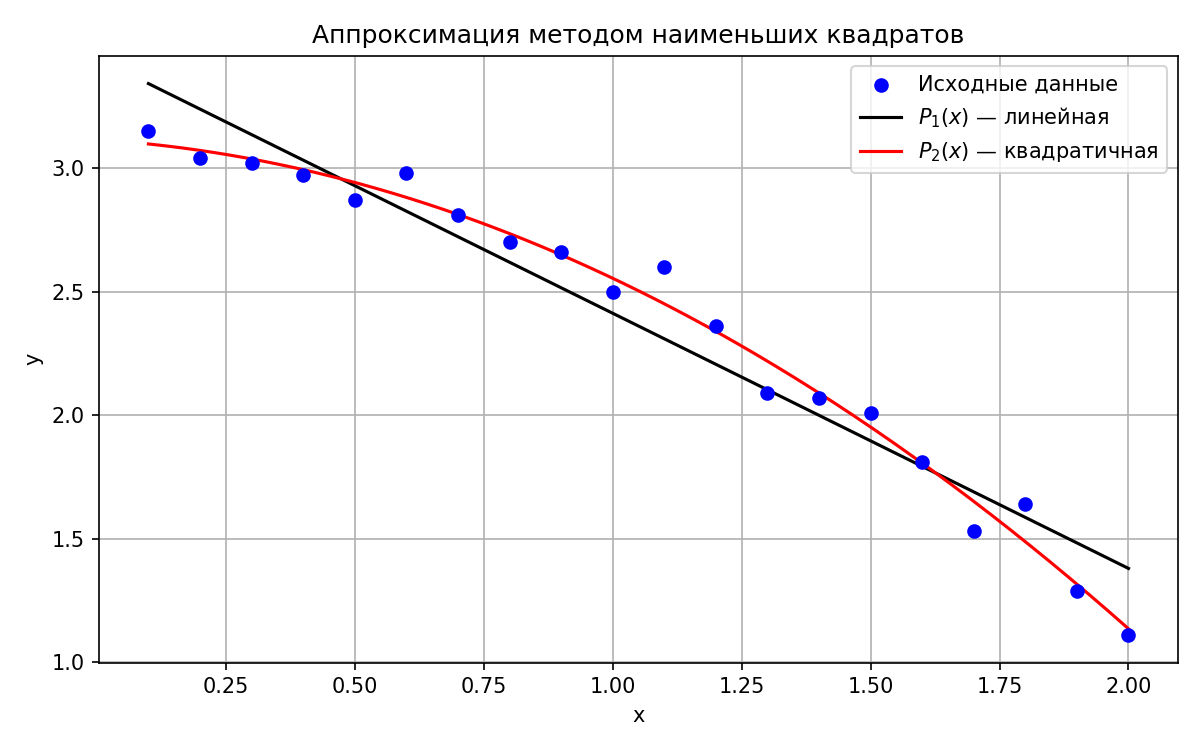
\includegraphics[width=0.85\textwidth]{approximation.png}
\caption{Графики исходных данных и аппроксимирующих полиномов.}
\label{fig:approx}
\end{figure}